\documentclass[../main.tex]{subfiles}

\begin{document}

\justifying

\section{Tabulación de potencial de dos cuerpos}

\paragraph{Objetivo} Aprender a usar el comando \verb|pair style table|.

\subsection{Descripción de la simulación}

Se coloca una partícula en el centro de la caja de simulación, \(\vec{r}_1 = (0,0,0)\).
Se coloca una segunda partícula a una distancia de \num{0.75} de la partícula central, \(\vec{r}_2 = (-0.75,0,0)\).
Usando el comando \verb|fix move| se mueve la segunda partícula a velocidad constante de \num{0.1}, \(\vec{v}_2 = (0.1,0,0)\), hacia el centro de la caja.
El paso temporal es de \num{1d-3}.
El número de pasos es \num{4500}, obteniendo una simulación de \num{4.5} unidades temporales.

Cada interacción entre dos partículas, se le asigna el siguiente potencial
\begin{gather}
    U_{\mathrm{patch}} = 
    \left\{
    \begin{array}{lc}
        2\epsilon_{ij}\left( \frac{1}{2}\left(\frac{D_p}{r_{ij}}\right)^{4}-1\right)\exp\left[\frac{D_{p}}{r_{ij}-r_{c}}+2\right]  & r_{ij}\in\qty[0,r_c] \\
        0 & r_{ij}>r_c
    \end{array}
    \right.
\end{gather}

La distancia entre los centros de las partícula está representada por \(r_{ij}\).
El parámetro \(\epsilon_{ij}\) controla el mínimo del potencial.
\(D_p\) es el diámtero de las partículas\footnote{La distancia entre los centros de las partículas esféricas.}.
El parámtero \(r_c\) es la distancia de corte definida en términos del diámetro de las partículas, \(r_c = 1.5 D_{p}\).

\begin{figure}[!ht]
    \centering
    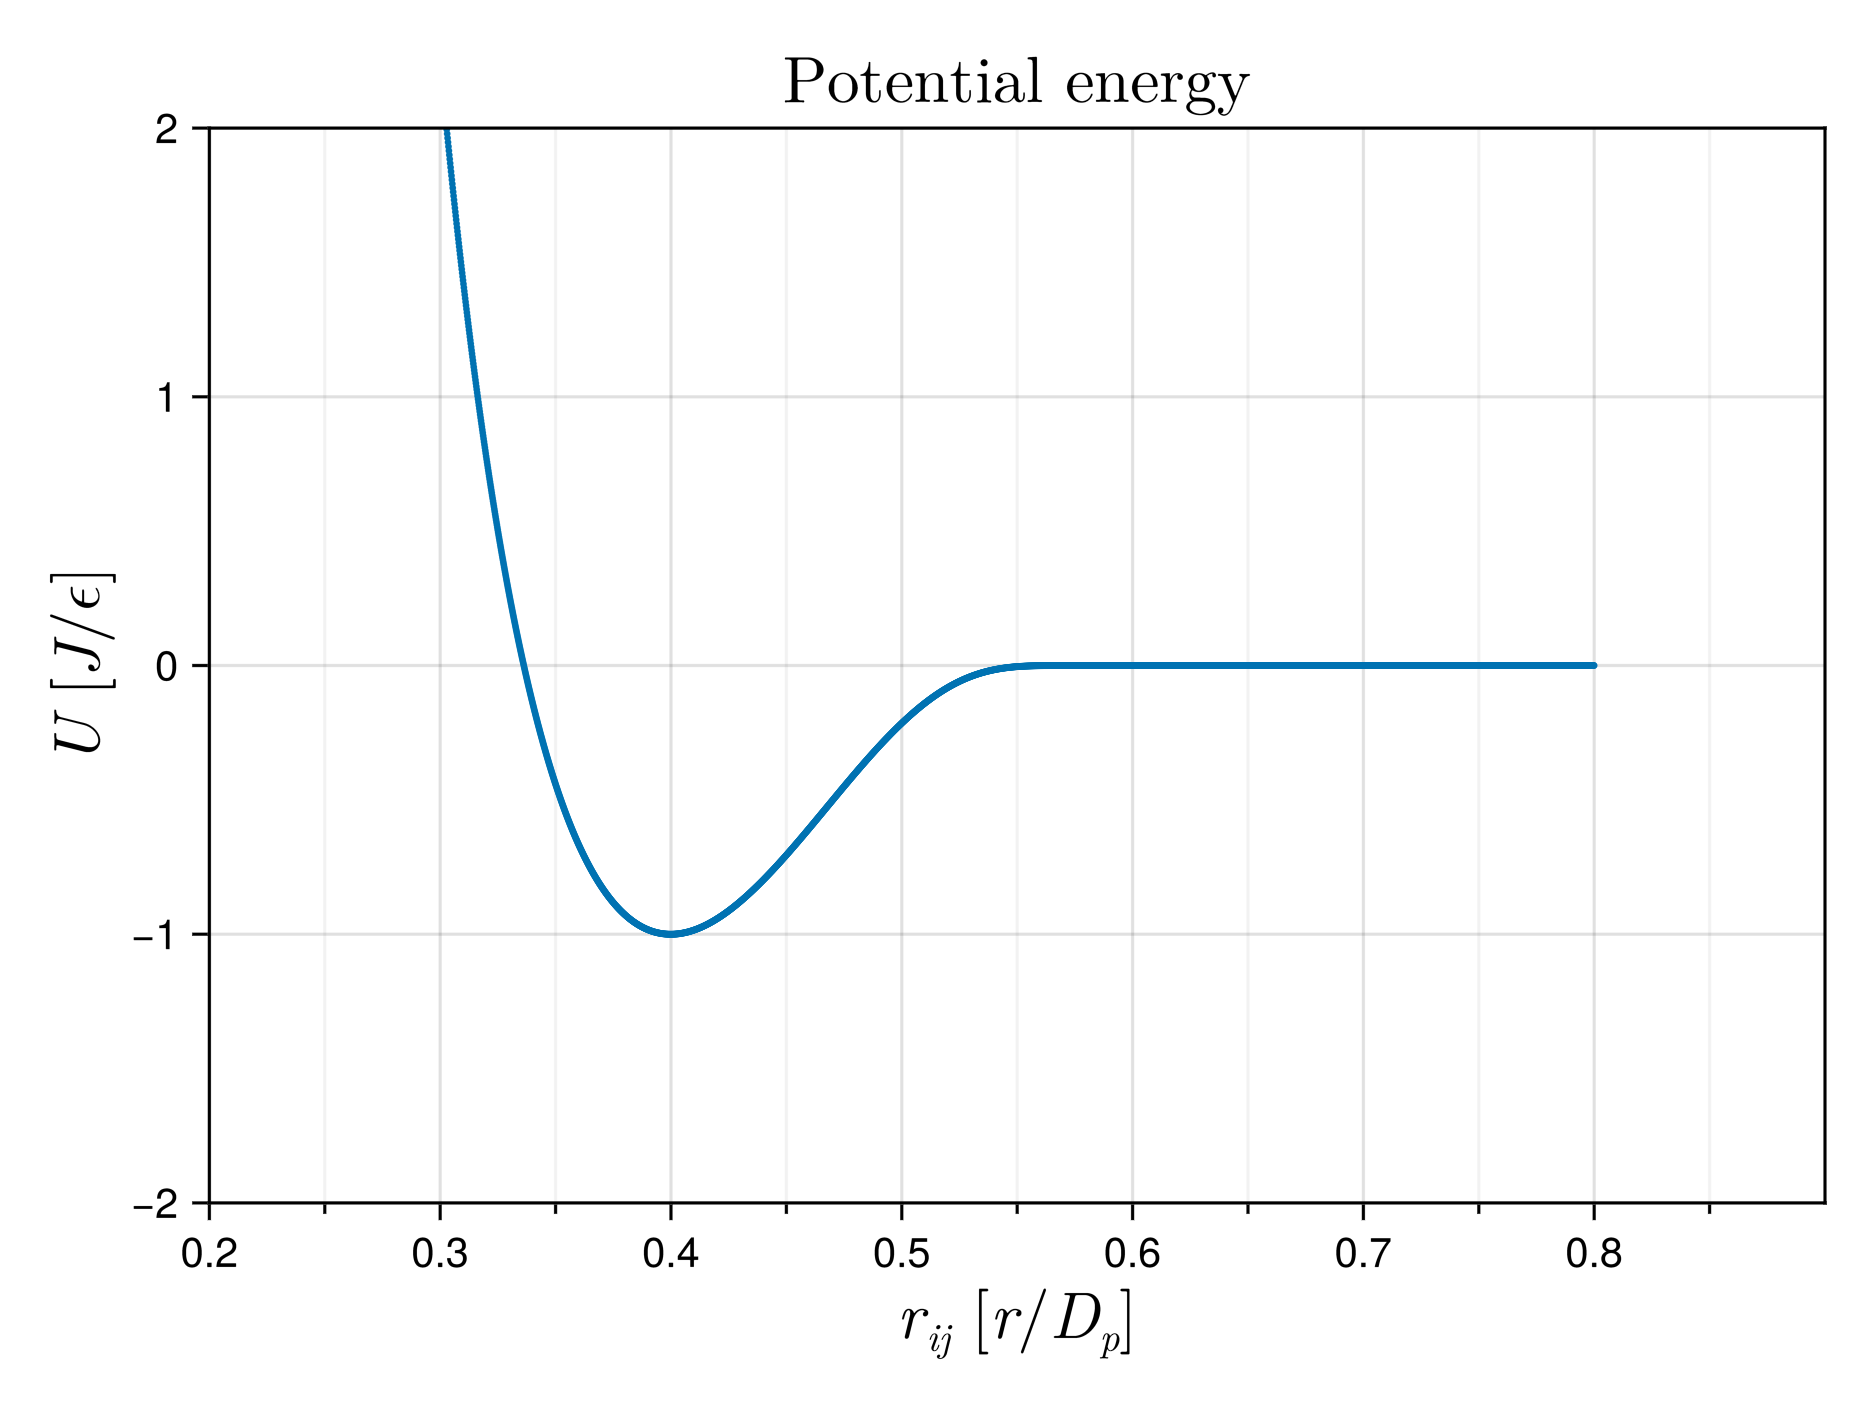
\includegraphics[width=0.8\textwidth]{../Figures/fig_Patchpot.png}
    \caption{Grafica del potencial de interacción entre \emph{patches}.
        \(\epsilon_{ij} = 1.0\), \( D_{p} = 0.4 \).
    }\label{fig:UpatchTeo}
\end{figure}

En el script de LAMMPS se registra la energía potencial con los siguientes comandos, \verb|compute ep all pe| y \verb|potAtom all pe/atom pair|.

\newpage

\section{Directory: 2026-02-05-140904}

\paragraph{Objetivo} Analizar la tabulación del potencial de interacción entre patches $U_\mathrm{patch}$ en LAMMPS.

\subsection{Resultados}

En la grafica~\ref{fig:2_Upotpartcor} se muestra la energía potencial registrada por el comand \verb|pe/atom|.
Hace sentido que las dos partículas tengan la misma forma del potencial.

\begin{figure}[ht]
    \centering
    
\includegraphics[width=0.75\textwidth]{../Figures/2026-02-05-140904/corr/fig_pot.png}
    \caption{Evolución temporal de la energía potencial en cada partícula y la evolución temporal de la distancia entre partículas.
    En el panel de arriba es la evolución temporal de la partícula qué está en el centro y en el panel de abajo es la evolución temporal de la energía potencial de la partícula que se está acercando.
    En el panel de en medio es la evolución temporal de la distancia entre partículas.}\label{fig:2_Upotpartcor}
\end{figure}


\begin{figure}[ht]
    \centering
    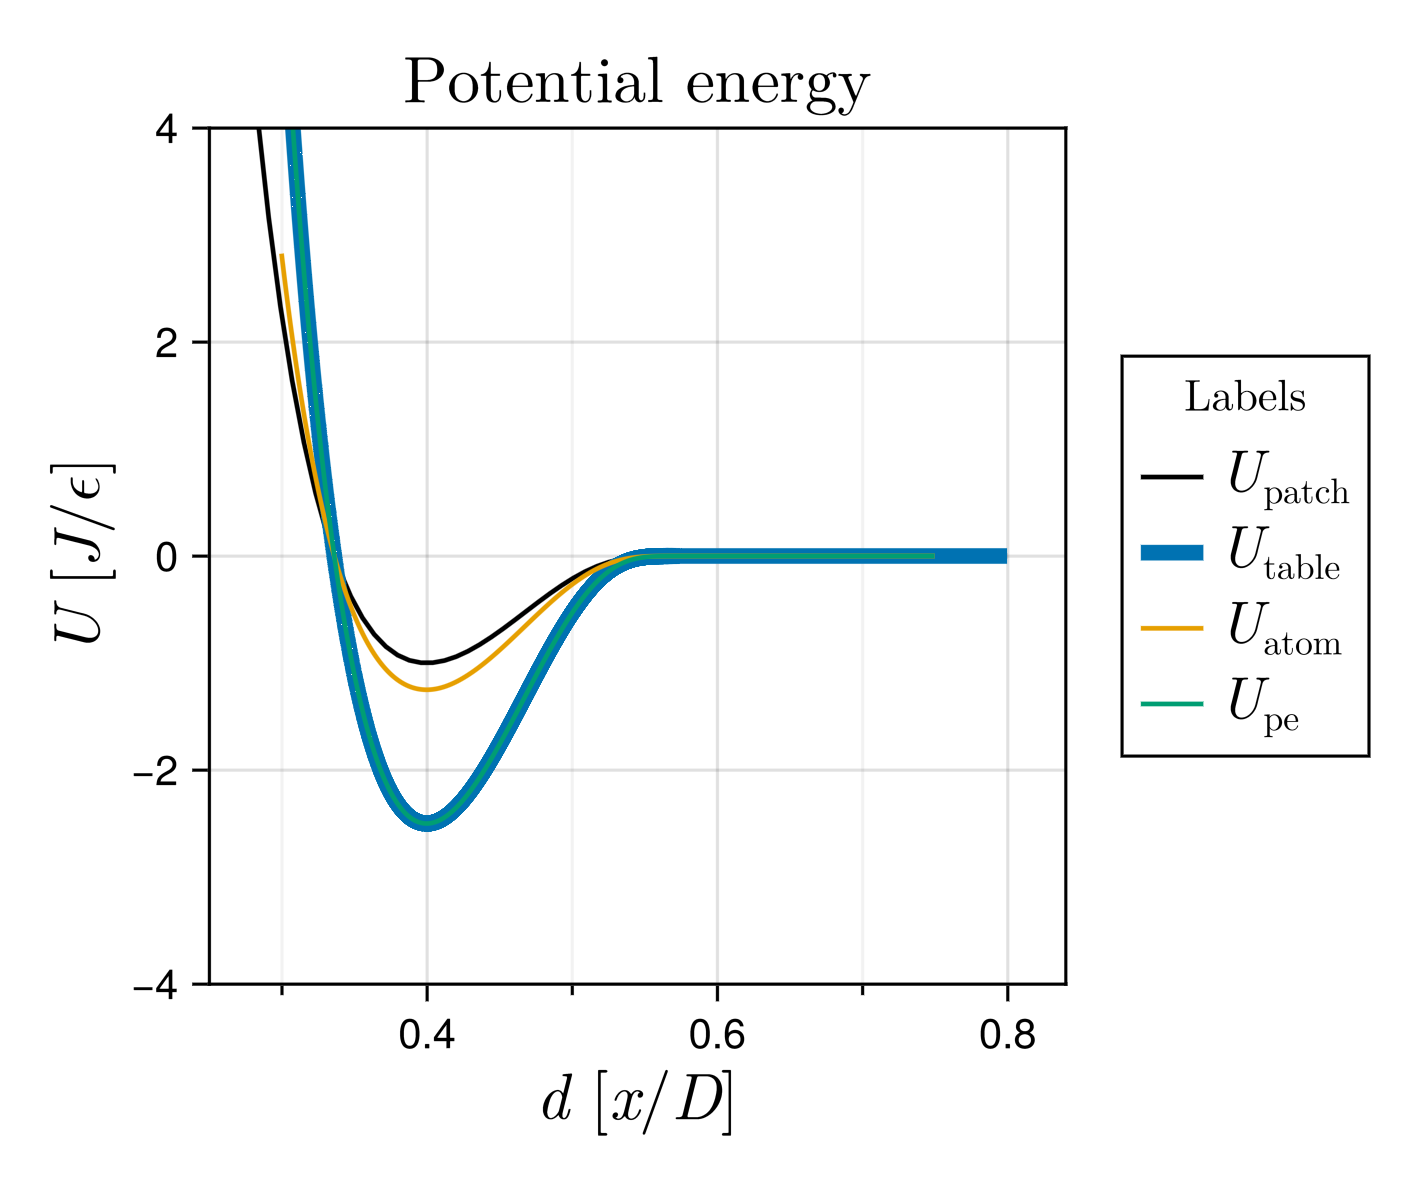
\includegraphics[width=0.8\textwidth]{../Figures/2026-02-05-140904/fig_potUComp.png}
    \caption{Comparación de la energía potencial entre la simulación y la forma algebráica.}\label{fig:3_UpotCompcor}
\end{figure}

\newpage

\subsection{Análisis/comentarios de datos corregidos}

En la figura~\ref{fig:3_UpotCompcor} se muestra una comparación entre 
la energía potencial de referencia (figura~\ref{fig:UpatchTeo}) marcada con un línea de color negro,
la energía registrada en la tabla del potencial marcada con una línea ancha de color azúl,
la energía registrada por el comando \verb|pe/atom| marcada con una línea de color amarillo y 
la energía resgistrada por el comando \verb|pe| marcada por una línea de color verde.

La tabulación tiene tiene un mayor pozo de potencial indicando que hay un error, porque se espera que el pozo de potencial sea igual a \num{1.0}.
Por otro lado, la energía potencial registrada por \verb|pe| coincide con con la energía potencial de la tabla, mientrás que la energía potencial registrada por \verb|pe/atom| tiene un menor pozo de potencial que coincide con la mitad del pozo de potencial registrados por \verb|pe|, \num{1.25}.
%Otra diferencia entre los potenciales, es la rapidez con la tienden a $\inty$ cuando $U>0$.





\newpage

\section{Directory: 2026-02-09-104056}

\paragraph{Objetivo} Hacer que el pozo de potencial sea igual a \num{1}.

\subsection{Resultados}

\begin{figure}[!ht]
    \centering
    
\includegraphics[width=0.8\textwidth]{../Figures/2026-02-09-104056/fig_potUComp.png}
    \caption{Comparación de la energía potencial entre la simulación y la forma algebráica.}
\end{figure}


\subsection{Comentarios}
\marginpar{
No entiendo porque lammps registra que el pozo de potencial es $0.5$?
Mi intuición es el \emph{style} que tiene el comando \verb|pair_style table| es \emph{linear} y hace es: 
\emph{For the linear style, the distance R is used to find the 2 surrounding table values from which an energy or force is computed by linear interpolation.}

Mientrás revisaba el código me di cuenta qué la declaración del comando estaba des-actualizado: \verb|table/omp linear 5000000|, cuando debería de marca \num{1000000}.
Cambiaré ese comando para ver si se arregla.
Sí no se arregla, exploraré lo los \emph{style}.
}
Cambié lo siguiente en el script de la tabulación de LAMMPS: \verb|eps=1.0| y \verb|rmin=sig/2|.

No entiendo que pasó.
Modifiqué el parámetro de la tabulación para que en la tabla sea igual a \num{1.0}, pero en el archivo, se regresó a tener un pozo de potencial de \num{2.5}.
Lo más raro, es que ahora, la energía potencial registrada por \verb|pe/atom| es igual al potencial de referencia.


\newpage

\section{Directory: 2026-02-10-114759}

\marginnote{
Se cambio el script de LAMMPS para simplificar las cosas.
Se retiro el patch del CL.
Se redujo la cantidad de puntos de tabulación, de \num{1d6} a \(2^{12} (4096)\).
}

\paragraph{Objetivo} Corregir la tabulación. 

\subsection{Resultados}

\begin{figure}[!ht]
    \centering
    
\includegraphics[width=0.8\textwidth]{../Figures/2026-02-10-114759/fig_potUComp.png}
    \caption{Comparación de la energía potencial entre la simulación y la forma algebráica.}
\end{figure}

\subsection{Comentarios}

Ahora ya coincide el potencial de referencia con el potencial de la tabla y la energía potencial registrada por el comando \verb|pe|.
Todo parece indicar que la energía potencial registrado por el comando \verb|pe/atom| hace su propia cosa.
Primero, el pozo del potencial está dividido en dos.
La \emph{forma algebráica} parece mantenerse, pero hay diferencia cuando el potencial tiende a \(\infty\).
Posiblemente se haga un tipo de interpolación.

\subsection{Dudas}

\paragraph{Qué pasa con una tercera partícula?} El potencial registrado por \verb|pe| se mantendrá igual que el potencial de referencia y la energía potencial de cada partícula será menor.

\paragraph{Qué pasa cuando se usa el Velocity Verlet?} Se obtendrán resultados similares cuando se empiecé a usar dinámica newtoniana?

\end{document}
